\subsection{Comparación de duración dentro del bloque A}
\label{sec:duracion_a}
La Tabla~\ref{tab:resultados} resume las duraciones completas de DAGMan por condición \citep{htcondortiming}. La Figura~\ref{fig:tiempos_pipeline} muestra las tres ejecuciones de cada agrupación del pipeline. Los envíos siguieron un orden fijo y las repeticiones de configuraciones distintas no forman pares temporales.

\begin{figure}[htbp]
\caption{Duraciones individuales y medianas del pipeline}
\label{fig:tiempos_pipeline}
\centering
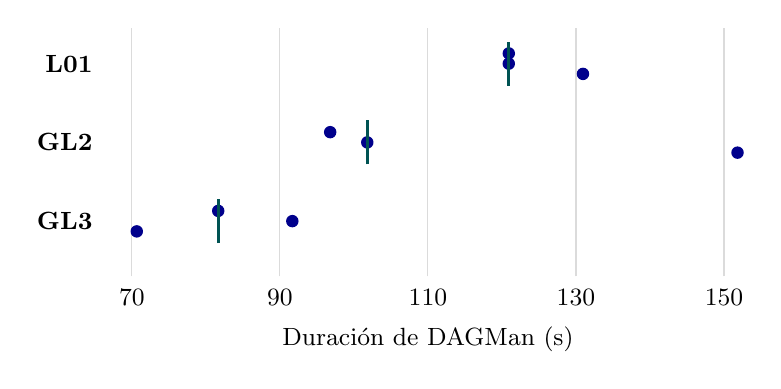
\begin{tikzpicture}[x=0.094cm,y=1cm,font=\small]
\foreach \x in {70,90,110,130,150} {
\draw[gray!28] (\x,0.30)--(\x,3.45);
\node[below] at (\x,0.26) {\x};
}
\node at (110,-0.50) {Duración de DAGMan (s)};
\foreach \y/\name in {3/L01,2/GL2,1/GL3} {
\node[left,font=\small\bfseries] at (66,\y) {\name};
}
\foreach \x/\y in {130.947/2.87,120.922/3.00,120.925/3.13,151.830/1.87,101.803/2.00,96.793/2.13,70.658/0.87,91.678/1.00,81.666/1.13} {
\fill[blue!55!black] (\x,\y) circle (2.25pt);
}
\foreach \x/\y in {120.925/3,101.803/2,81.666/1} {
\draw[teal!65!black,very thick] (\x,\y-0.28)--(\x,\y+0.28);
}
\end{tikzpicture}
\par\smallskip\footnotesize Puntos, ejecuciones individuales. Trazo, mediana. La separación vertical dentro de una misma fila facilita distinguir puntos próximos.
\end{figure}

Las medianas de L01 y GL2 fueron 120,925 y 101,803 s. El máximo de GL2, 151,830 s, superó el de L01, 130,947 s. Las tres duraciones de GL3 quedaron por debajo del mínimo de L01.

Para el archivo compartido, las medianas de AC1, AC2 y AC4 fueron 137,194, 126,833 y 105,815 s, a la vez que bajaron los bytes entregados. Los rangos de AC1 y AC2 se solapan. D02 y GD4 conservaron el volumen y sus medianas fueron 130,967 y 100,836 s. Las diferencias de duración describen las configuraciones completas. La agrupación también cambia el número de jobs, por lo que el diseño no aísla el efecto de los bytes.

\subsection{Criterios para recomendar una configuración}
\label{sec:decisiones_a}
La recomendación depende del criterio del usuario. Para reducir bytes científicos se comparan observados bajo trabajo y fronteras equivalentes. Cuando el requerido positivo es común, un DME mayor corresponde a un volumen observado menor. Si la ubicación cambia, el valor de DME se interpreta con los dos volúmenes y el desglose por destino. En ninguna de estas comparaciones el valor de la razón reemplaza la duración registrada.



\subsection{Sobrecosto de instrumentación}
\label{sec:costo_a}
La medición utiliza los planes y registros nativos de Pegasus y HTCondor. La exportación del historial y el cálculo de DME ocurren después del workflow; sus tiempos no estiman el costo de generar registros durante la ejecución. En la campaña, las medianas de exportación y análisis fueron 0,128 y 0,214 s, respectivamente, con el ejecutable de entonces. No se suman como mediana conjunta ni se atribuyen al código actual. El costo de captura nativa no quedó aislado y limita el cumplimiento de OE4. Los registros individuales se conservan en los materiales.

